% Options for packages loaded elsewhere
% Options for packages loaded elsewhere
\PassOptionsToPackage{unicode}{hyperref}
\PassOptionsToPackage{hyphens}{url}
\PassOptionsToPackage{dvipsnames,svgnames,x11names}{xcolor}
%
\documentclass[
  letterpaper,
  DIV=11,
  numbers=noendperiod]{scrartcl}
\usepackage{xcolor}
\usepackage[margin=0.75in]{geometry}
\usepackage{amsmath,amssymb}
\setcounter{secnumdepth}{-\maxdimen} % remove section numbering
\usepackage{iftex}
\ifPDFTeX
  \usepackage[T1]{fontenc}
  \usepackage[utf8]{inputenc}
  \usepackage{textcomp} % provide euro and other symbols
\else % if luatex or xetex
  \usepackage{unicode-math} % this also loads fontspec
  \defaultfontfeatures{Scale=MatchLowercase}
  \defaultfontfeatures[\rmfamily]{Ligatures=TeX,Scale=1}
\fi
\usepackage{lmodern}
\ifPDFTeX\else
  % xetex/luatex font selection
\fi
% Use upquote if available, for straight quotes in verbatim environments
\IfFileExists{upquote.sty}{\usepackage{upquote}}{}
\IfFileExists{microtype.sty}{% use microtype if available
  \usepackage[]{microtype}
  \UseMicrotypeSet[protrusion]{basicmath} % disable protrusion for tt fonts
}{}
\makeatletter
\@ifundefined{KOMAClassName}{% if non-KOMA class
  \IfFileExists{parskip.sty}{%
    \usepackage{parskip}
  }{% else
    \setlength{\parindent}{0pt}
    \setlength{\parskip}{6pt plus 2pt minus 1pt}}
}{% if KOMA class
  \KOMAoptions{parskip=half}}
\makeatother
% Make \paragraph and \subparagraph free-standing
\makeatletter
\ifx\paragraph\undefined\else
  \let\oldparagraph\paragraph
  \renewcommand{\paragraph}{
    \@ifstar
      \xxxParagraphStar
      \xxxParagraphNoStar
  }
  \newcommand{\xxxParagraphStar}[1]{\oldparagraph*{#1}\mbox{}}
  \newcommand{\xxxParagraphNoStar}[1]{\oldparagraph{#1}\mbox{}}
\fi
\ifx\subparagraph\undefined\else
  \let\oldsubparagraph\subparagraph
  \renewcommand{\subparagraph}{
    \@ifstar
      \xxxSubParagraphStar
      \xxxSubParagraphNoStar
  }
  \newcommand{\xxxSubParagraphStar}[1]{\oldsubparagraph*{#1}\mbox{}}
  \newcommand{\xxxSubParagraphNoStar}[1]{\oldsubparagraph{#1}\mbox{}}
\fi
\makeatother


\usepackage{longtable,booktabs,array}
\usepackage{calc} % for calculating minipage widths
% Correct order of tables after \paragraph or \subparagraph
\usepackage{etoolbox}
\makeatletter
\patchcmd\longtable{\par}{\if@noskipsec\mbox{}\fi\par}{}{}
\makeatother
% Allow footnotes in longtable head/foot
\IfFileExists{footnotehyper.sty}{\usepackage{footnotehyper}}{\usepackage{footnote}}
\makesavenoteenv{longtable}
\usepackage{graphicx}
\makeatletter
\newsavebox\pandoc@box
\newcommand*\pandocbounded[1]{% scales image to fit in text height/width
  \sbox\pandoc@box{#1}%
  \Gscale@div\@tempa{\textheight}{\dimexpr\ht\pandoc@box+\dp\pandoc@box\relax}%
  \Gscale@div\@tempb{\linewidth}{\wd\pandoc@box}%
  \ifdim\@tempb\p@<\@tempa\p@\let\@tempa\@tempb\fi% select the smaller of both
  \ifdim\@tempa\p@<\p@\scalebox{\@tempa}{\usebox\pandoc@box}%
  \else\usebox{\pandoc@box}%
  \fi%
}
% Set default figure placement to htbp
\def\fps@figure{htbp}
\makeatother





\setlength{\emergencystretch}{3em} % prevent overfull lines

\providecommand{\tightlist}{%
  \setlength{\itemsep}{0pt}\setlength{\parskip}{0pt}}



 


\KOMAoption{captions}{tableheading}
\usepackage{../latex_packages/abbreviations}
\usepackage{fancyhdr}
\pagestyle{fancy}
\let\headrule\empty
\let\footrule\empty
\lhead{{\bfseries CSC\,413}}
\chead{{\bfseries Exercises - Week 8}}
\rhead{{\bfseries Shkurti / Gilitschenski}}
\lfoot{{}}
\cfoot{{\thepage}}
\rfoot{{}}
\makeatletter
\@ifpackageloaded{caption}{}{\usepackage{caption}}
\AtBeginDocument{%
\ifdefined\contentsname
  \renewcommand*\contentsname{Table of contents}
\else
  \newcommand\contentsname{Table of contents}
\fi
\ifdefined\listfigurename
  \renewcommand*\listfigurename{List of Figures}
\else
  \newcommand\listfigurename{List of Figures}
\fi
\ifdefined\listtablename
  \renewcommand*\listtablename{List of Tables}
\else
  \newcommand\listtablename{List of Tables}
\fi
\ifdefined\figurename
  \renewcommand*\figurename{Figure}
\else
  \newcommand\figurename{Figure}
\fi
\ifdefined\tablename
  \renewcommand*\tablename{Table}
\else
  \newcommand\tablename{Table}
\fi
}
\@ifpackageloaded{float}{}{\usepackage{float}}
\floatstyle{ruled}
\@ifundefined{c@chapter}{\newfloat{codelisting}{h}{lop}}{\newfloat{codelisting}{h}{lop}[chapter]}
\floatname{codelisting}{Listing}
\newcommand*\listoflistings{\listof{codelisting}{List of Listings}}
\makeatother
\makeatletter
\makeatother
\makeatletter
\@ifpackageloaded{caption}{}{\usepackage{caption}}
\@ifpackageloaded{subcaption}{}{\usepackage{subcaption}}
\makeatother
\usepackage{bookmark}
\IfFileExists{xurl.sty}{\usepackage{xurl}}{} % add URL line breaks if available
\urlstyle{same}
\hypersetup{
  colorlinks=true,
  linkcolor={blue},
  filecolor={Maroon},
  citecolor={Blue},
  urlcolor={Blue},
  pdfcreator={LaTeX via pandoc}}


\author{}
\date{}
\begin{document}


\subsection{Exercise 1 - RNN for Sentiment
Analysis}\label{exercise-1---rnn-for-sentiment-analysis}

Suppose we are training a vanilla RNN like below to determine whether a
sentence expresses positive or negative sentiment. This RNN will be a
character-level RNN where \(x^{(1)}, \ldots, x^{(T)}\) is the sequence
of input characters. The RNN is given as follows: \begin{align*}
h^{(t)} &= \tanh\li(U x^{(t)} + W h^{(t-1)} + b\ri) \\
y &= \sigma\li(V h^{(T)} + d\ri)
\end{align*}

\begin{enumerate}
\def\labelenumi{(\alph{enumi})}
\item
  How many times do we need to apply the weight matrix \(U\), \(W\), and
  \(V\)?
\item
  What are the shapes of the matrices \(U\), \(W\), and \(V\)?
\item
  How many addition and multiplication operations are required to make a
  prediction? You can assume that no addition and multiplications are
  performed when applying the tanh and sigmoid activation functions.
\end{enumerate}

\subsubsection{Solution}\label{solution}

\begin{enumerate}
\def\labelenumi{(\alph{enumi})}
\item
  We will need to compute \(h^{(t)}\) for \(t = 1, \ldots, T\). Each of
  this computation requires applying the weight matrices \(W\) and \(T\)
  once. The matrix \(V\) is only applied once at the end. Therefore, we
  need to apply \(W\) and \(U\) \(T\) times each and \(V\) once.
\item
  The shape of \(U\) is \(d_h \times d_x\), the shape of \(W\) is
  \(d_h \times d_h\), and the shape of \(V\) is \(d_y \times d_h\),
  where \(d_h\) is the dimensionality of the \(h^{(i)}\)
  (i.e.~\(h^{(i)}\in\R^{d_h}\)), \(d_x\) is the dimensionality of the
  inputs \(x^{(i)}\), and \(d_y\) is the dimensionality of the ouput
  \(y\).
\item
  For each of the \(T\) steps, we need to perform two matrix-vector
  multiplications (one for \(Ux^{(i)}\) and one for \(Uh^{(i)}\)) and
  two vector additions. To compute the output, we need one additional
  matrix-vector multiplication and one vector addition.
\end{enumerate}

\subsection{Exercise 2 - Scalar RNN}\label{exercise-2---scalar-rnn}

Suppose we have the following vanilla RNN network, where the inputs and
hidden units are scalars. \begin{align*}
h^{(t)} &= \tanh\li(w \cdot h^{(t-1)} + u \cdot x^{(t-1)} + b_h\ri) \\
y &= \sigma\li(v \cdot h^{(T)} + b_y\ri)
\end{align*}

\begin{enumerate}
\def\labelenumi{(\alph{enumi})}
\item
  Show that if \(|w| < 1\), and the number of time steps \(T\) is large,
  then the gradient \(\frac{\partial y}{\partial x^{(0)}}\) vanishes.
\item
  Why is the result from Part (a) troubling?
\end{enumerate}

\subsubsection{Solution}\label{solution-1}

\begin{enumerate}
\def\labelenumi{(\alph{enumi})}
\item
  To make the sequence length \(T\) explicit in the notation, we will
  write \(y\) instead of \(y_T\). Formally, what we have to show is \[
  |w|<1 \implies \lim_{T\to\infty} \fr{\partial y_T}{\partial x^{(0)}} = 0 .
  \] For the proof, we expand the derivative of \(y_T\) with respect to
  \(x^{(0)}\) using the chain rule: \[
  \begin{aligned}
  \fr{\partial y_T}{\partial x^{(0)}} 
    & = \si'\li(v \cdot h^{(T)} + b_y\ri) 
      \cdot v \cdot \fr{\partial h^{(T)}}{\partial x^{(0)}} \\
    & = 
    \si'\li(v \cdot h^{(T)} + b_y\ri) 
      \cdot v 
      \cdot 
        \underbrace{
          \tanh'\li(w \cdot h^{(T-1)} + u \cdot x^{(T-1)} + b_h\ri)
        }_{A_{T-1}(x^{(0)})}
      \cdot w \cdot \fr{\partial h^{(T-1)}}{\partial x^{(0)}} \\
   & = \ldots \\
   & = \si'\li(v \cdot h^{(T)} + b_y\ri) 
      \cdot v 
      \cdot \prod_{t=2}^{T-1} A_{t}(x^{(0)})
      \cdot w^{T-1} \cdot \fr{\partial h^{(1)}}{\partial x^{(0)}} .\\
  \end{aligned}
  \] Using this, we can analyze the absolute value of the derivative
  \(\partial y_T/\partial x^{(0)}\). For \(\tanh\) and \(\si\), the
  absolute value of their respective derivatives is bounded by \(1\).
  Thus, we have \[
  \begin{aligned}
  \li|\fr{\partial y_T}{\partial x^{(0)}} \ri|
  & = 
  \underbrace{
    \li|\si'\li(v \cdot h^{(T)} + b_y\ri) \ri|
  }_{\leq 1}
  \cdot |v| 
  \cdot \prod_{t=2}^{T-1} 
    \underbrace{\li| A_{t}(x^{(0)}) \ri|}_{\leq 1}
  \cdot \li|w^{T-1}\ri| 
  \cdot \li|\fr{\partial h^{(1)}}{\partial x^{(0)}}\ri| \\
  & \leq |v| 
  \cdot \li|w^{T-1}\ri| 
  \cdot \li|\fr{\partial h^{(1)}}{\partial x^{(0)}}\ri| \\
  \end{aligned}
  \] Because \(|w|<1\), this converges to \(0\) as \(T\to\infty\) and
  thus \(|\partial y_T/\partial x^{(0)}|\) also converges to \(0\),
  i.e.~the gradient vanishes.
\item
  It implies that in the considered setting, the input has no impact on
  the output.
\end{enumerate}

\subsection{Exercise 3 - RNN Addition}\label{exercise-3---rnn-addition}

In this problem, you will implement a recurrent neural network which
implements binary addition. The inputs are given as binary sequences,
starting with the \emph{least} significant binary digit. (It is easier
to start from the least significant bit, just like how you did addition
in grade school.) The sequences will be padded with at least one zero as
the most significant digit, so that the output length is the same as the
input length. For example, the problem \(100111 + 110010\), whose target
output value is \(1011001\), will be represented as follows:
\begin{align*}
\bf{x}^{(1)} = \begin{bmatrix}1 \\ 0\end{bmatrix},
\bf{x}^{(2)} = \begin{bmatrix}1 \\ 1\end{bmatrix},
\bf{x}^{(3)} = \begin{bmatrix}1 \\ 0\end{bmatrix},
\bf{x}^{(4)} = \begin{bmatrix}0 \\ 0\end{bmatrix},
\bf{x}^{(5)} = \begin{bmatrix}0 \\ 1\end{bmatrix},
\bf{x}^{(6)} = \begin{bmatrix}1 \\ 1\end{bmatrix},
\bf{x}^{(7)} = \begin{bmatrix}0 \\ 0\end{bmatrix}
\end{align*}

With the target output: \begin{align*}
y^{(1)} = 1,
y^{(2)} = 0,
y^{(3)} = 0,
y^{(4)} = 1,
y^{(5)} = 1,
y^{(6)} = 0,
y^{(7)} = 1,
\end{align*}

There are two input units corresponding to the two inputs, and one
output unit. Therefore, the pattern of inputs and outputs for this
example would be:

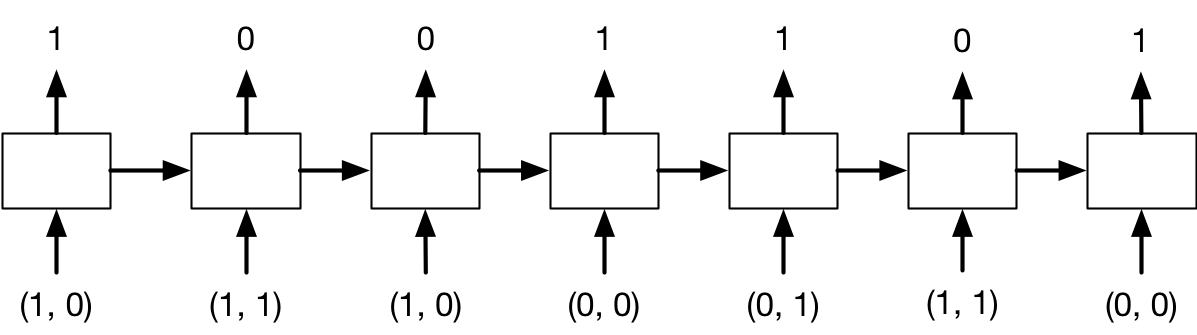
\includegraphics[width=3in,height=\textheight,keepaspectratio]{rnn-addition.png}

Design, by hand, the weights and biases for an RNN which has two input
units, three hidden units, and one output unit, which implements binary
addition as discussed above. All of the units use the hard threshold
activation function (\(f(x) = 1\) if \(x > 0\) and \(0\) otherwise). In
particular, specify weight matrices \(\mathbf{U}\), \(\mathbf{v}\), and
\(\mathbf{W}\), bias vector \(\mathbf{b}_{\mathbf{h}}\), and scalar bias
\(b_y\) for the following architecture: \begin{align*}
h^{(t)} &= f(\bf{W}h^{(t-1)} + \bf{U}\bf{x}^{(t)} + \bf{b_h}) \\
y^{(t)} &= f(\bf{v}^T h^{(t)} + b_y)
\end{align*}

\begin{enumerate}
\def\labelenumi{(\alph{enumi})}
\item
  What are the shapes of \(\mathbf{U}\), \(\mathbf{v}\), \(\mathbf{W}\),
  and \(\mathbf{b}_{\mathbf{h}}\)?
\item
  Come up with values for \(\mathbf{U}\), \(\mathbf{W}\), and
  \(\mathbf{b}_{\mathbf{h}}\). Justify your answer. \textbf{Hint:} When
  performing binary addition, in addition to adding up two digits in a
  column, we need to track whether there is a \textit{carry} digit from
  the previous column. We will choose one of the three units in
  \(\bf{h}^{(t)}\), say \(\bf{h}_2^{(t)}\), to represent this carry
  digit. You may also find it helpful to set \(\bf{h}_1\) to activate if
  the sum of the 3 digits is at least 1, \(\bf{h}_2\) to activate if the
  sum is at least 2, and \(\bf{h}_3\) to activate if the sum is at least
  3.
\item
  Come up with the values of \(\bf{v}\) and \(b_y\). Justify your
  answer.
\end{enumerate}

\subsubsection{Solution}\label{solution-2}

\begin{enumerate}
\def\labelenumi{(\alph{enumi})}
\item
  Since the inputs \(\bf{x}^{(t)}\) are \(2 \times 1\) and the hidden
  units \(\bf{h}^{(t)}\) are \(2 \times 1\), we should have:

  \begin{itemize}
  \tightlist
  \item
    \(\bf{W}\) is \(3 \times 3\)
  \item
    \(\bf{U}\) is \(3 \times 2\)
  \item
    \(\bf{b}_h\) is \(3 \times 1\)
  \item
    \(\bf{v}\) is \(3 \times 1\)
  \end{itemize}
\item
  We will follow the hint and implement the addition in our RNN such
  that:

  \begin{enumerate}
  \def\labelenumii{\arabic{enumii}.}
  \tightlist
  \item
    The first of our hidden units \(h_1^{(t)}\) is 1 if and only if the
    sum \(S^{(t)} \doteq x_1^{(t)} + x_2^{(t)} + c^{(t-1)} \geq 1\),
    where by \(c^{(t-1)}\) we denote a carry (\(\bf{h_2}^{(t-1)}\) from
    the previous addition). Note, these \(S^{(t)}\) and \(c^{(t-1)}\)
    are not variables of the model, merely our notation to help us to
    work out the solution.
  \item
    The \(h_2^{(t)}\) is 1 iff the sum \(S^{(t)} \geq 2\),
  \item
    and \(h_3^{(t)}\) is 1 iff the sum \(S^{(t)}\) is 3.
  \end{enumerate}

  Notice that the carry \(c^{(t-1)}\) is going to be 1 iff
  \(h_2^{(t-1)}=1\) and 0
  otherwise\footnote{We need to initialize $\mathbf{h}^{(0)}=\mathbf{0}$.},
  i.e.~when the previous addition was 2 or 3. Therefore to compute
  \(h_i^{(t)}\) we need to first compute the sum
  \(S^{(t)} = x_1^{(t)} + x_2^{(t)} + h_2^{(t-1)}\) and then offset it
  by \(-i+1\) so that after applying the hard threshold function we get
  the desired value as specified above. This can be achieved with the
  following set of parameters: \[
  \mathbf{U}= \begin{bmatrix}
      1 & 1 \\
      1 & 1 \\
      1 & 1 \end{bmatrix},\quad
  \mathbf{W}=\begin{bmatrix}
      0 & 1 & 0 \\
      0 & 1 & 0 \\
      0 & 1 & 0\end{bmatrix},\quad
  \mathbf{b_h}= \begin{bmatrix}
      -0.5 \\
      -1.5 \\
      -2.5 \end{bmatrix}. 
  \]
\item
  To compute the output \(y^{(t)}\) we need to check if the \(S^{(t)}\)
  is 1 or 3, that is, if either \(h_1^{(t)} = 1\) while all other hidden
  units are zero or all hidden units are 1. We can accomplish this by
  setting: \(\mathbf{v}=\begin{bmatrix} 1, -1, 1 \end{bmatrix}\) and
  \(b_y = -0.5\).
\end{enumerate}




\end{document}
